\documentclass[]{cv-lea}

\usepackage[italian, american]{babel}

\usepackage[autostyle]{csquotes}
%\usepackage{graphix}  

\usepackage{fontawesome}

\addbibresource{curriculum.bib}

\hypersetup{%
  colorlinks=false,% hyperlinks will be black
  linkbordercolor=red,% hyperlink borders will be red
  pdfborderstyle={/S/U/W 1}% border style will be underline of width 1pt
}

\newfontfamily{\FA}{FontAwesome Regular}


\begin{document}
\header{Léa}{Delay}{Master en kinésithérapie}
       
\begin{aside} % In the aside, each new line forces a line break
%\includegraphics[width=largeur]{nom du fichier}
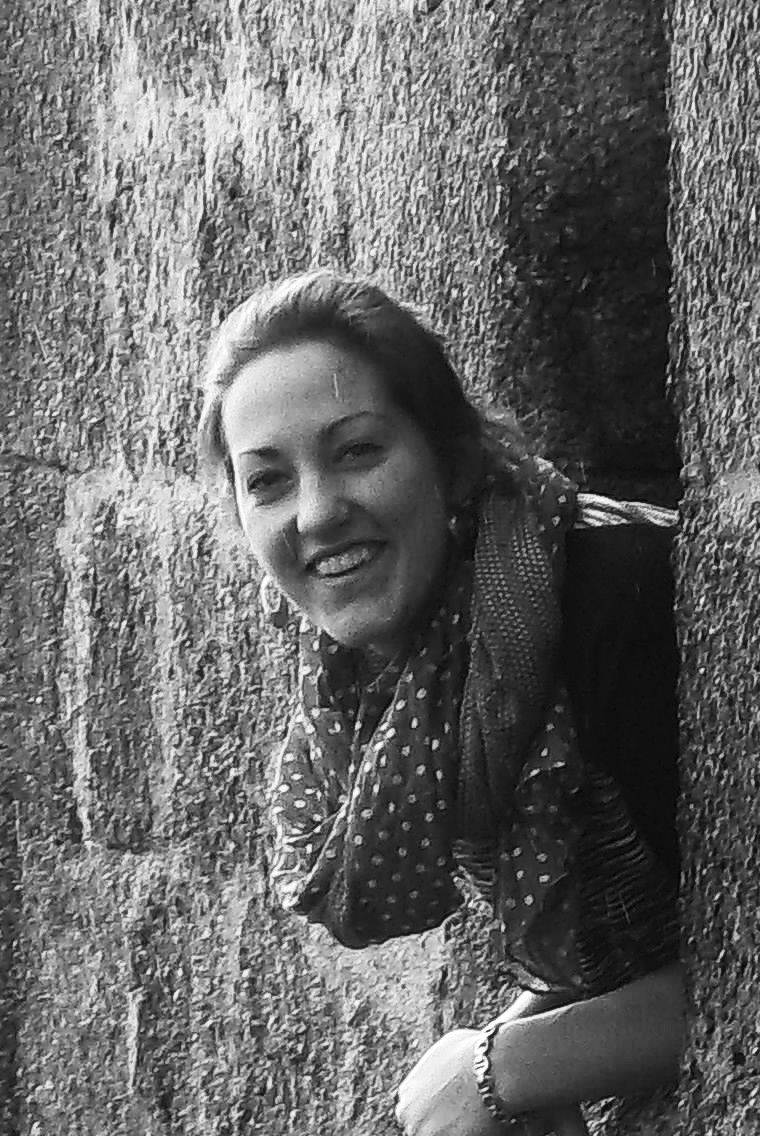
\includegraphics{img/delay_s}
\section{Contact}
Les combes
38780 Estrablin
France
~
+33 6 65 17 58 35
~
{\color{lightgray}{\FA \faEnvelope}} \href{mailto:delay.lea@gmail.com}{\footnotesize delay.lea@gmail.com}
\section{Langages}
Français : langue\\ maternelle
Anglais : scolaire
Espagnol :maîtrise convenable de la langue
Langue des Signes: Niveau 1.
\end{aside}


\section{Intérêts}
Diplômée en Master de Kinésithérapie au sein de la Haute École de la Province de Liège.
Durant mes études, j’ai eu la chance d’avoir des expériences de terrain grâce à de nombreux
stages. Au cours de ces expériences professionnelles j’ai appris à travailler en équipe, tout en développant mon sens de l’autonomie.

Je me suis investis dans la vie communautaire de l'école où j'ai effectué ma formation. J'ai été présidente du Comité KinErgo 2014-2015 qui est en charge de récolter les fonds pour financer le voyage de fin d'étude des étudiants de dernières années en Kinésithérapie et Ergothérapie de l'école. J'ai été membre du conseil étudiant de la Haute École de la Province de Liège, en charge de représenter les étudiants face à l'administration.

J'ai été trésorière adjointe en 2009-2010, de l'Association Loisir et Culture de mon établissement.
Ces expériences ont été riches en enseignement tant au niveau du sens des responsabilités
que de celui de l'organisation.

J’aime : les voyages, lire pendant des heures, les sports d’équipe et la course à pied.

\section{Cursus Universitaire}

\begin{entrylist}
%------------------------------------------------
\entry
{2014-2015}
{Master en kinésithérapie}
{Haute École de la Province de Liège, BE}
{\emph{Distinction, prix de la citoyenneté}}
%------------------------------------------------
\end{entrylist}
\begin{entrylist}
%------------------------------------------------
\entry
{2011-2014}
{Baccalauréat en kinésithérapie}
{Haute École de la Province de Liège, BE}
{\emph{Distinction, prix du Fairplay}}
%------------------------------------------------
\end{entrylist}
\begin{entrylist}
%------------------------------------------------
\entry
{2010-2011}
{L1 Sciences et Techniques des Activités Physiques et Sportives}
{Université Joseph Fourier, Grenoble, FR}
{\emph{Spécialité Sportive Basket-ball}}
%------------------------------------------------
\end{entrylist}

\section{Expériences professionnelles}

\begin{entrylist}
%------------------------------------------------
\entry
{2015-2016}
{Kinésithérapeute au sein de l'Union Beynoise Hanball}
{Beyne-Heusay, BE}
{\emph{Club Sportif, indépendante}\\
Prise en charge des soins pour l'ensemble des membres actifs et en particulier l'équipe senior qui militait en Division 1 nationale au cours de la saison 2015-2016.\\
Techniques mobilisées : Pose de Kinesio Tape, suivi du sportif, intervention rapide sur le terrain.
}
\end{entrylist}
%------------------------------------------------
\begin{entrylist}
%------------------------------------------------
\entry
{2016}
{Maison médicale de la Passerelle}
{Liège, BE}
{\emph{Remplacement, indépendante (3 semaines)}\\
Rééducation et prise en charge de patients à domicile et en cabinet, et
sensibilisation aux valeurs défendues par les maisons médicales.
}
\end{entrylist}
%------------------------------------------------
\begin{entrylist}
%------------------------------------------------
\entry
{2016}
{Maison médicale du Cadran}
{Liège, BE}
{\emph{Remplacement, indépendante (1 semaine)}\\
Rééducation et prise en charge de patients à domicile et en cabinet.
}
\end{entrylist}
%------------------------------------------------
\begin{entrylist}
%------------------------------------------------
\entry
{2015-2016}
{Cabinet privée de Philippe LECLERCQ}
{Liège, BE}
{\emph{Assistanat, indépendante (29 semaines)}\\
Rééducation et prise en charge de patients à domicile, cabinet et centre pour adultes handicapés.
}
\end{entrylist}
%------------------------------------------------
\begin{entrylist}
%------------------------------------------------
\entry
{2015}
{Maison médicale de Tilleur}
{Saint Nicolas, BE}
{\emph{Remplacement, salariée (2 semaines)}\\
Rééducation et prise en charge de patients à domicile et en cabinet.
}
\end{entrylist}
%------------------------------------------------
\begin{entrylist}
%------------------------------------------------
\entry
{2015}
{Maison médicale de l'Herma}
{Liège, BE}
{\emph{Remplacement, salariée (6 semaines)}\\
Rééducation et prise en charge de patients à domicile et en cabinet.
}
\end{entrylist}
%------------------------------------------------
\begin{entrylist}
\entry
{2015}
{Maison médicale du Laveu}
{Liège, BE}
{\emph{Remplacement, salariée (10 semaines)}\\
Rééducation et prise en charge de patients à domicile et en cabinet.
}
\end{entrylist}
%------------------------------------------------
\begin{entrylist}
\entry
{2015}
{Maison médicale de Ougrée}
{Saint Nicolas, BE}
{\emph{Remplacement, salariée (1 semaine)}\\
Rééducation et prise en charge de patients à domicile et en cabinet.
}
\end{entrylist}
%------------------------------------------------
\begin{entrylist}
\entry
{2015}
{Maison de repos et de soins "Le Temps des cerisiers"}
{Saint Nicolas, BE}
{\emph{Remplacement, salariée (1 semaine)}\\
Rééducation et prise en charge de patients âgés fragiles.
}
\end{entrylist}
%------------------------------------------------
\begin{entrylist}
\entry
{2015}
{Maison médicale "Les Houlpays"}
{Liège, BE}
{\emph{Remplacement, salariée (4 semaines)}\\
Rééducation et prise en charge de patients à domicile et en cabinet.\\
Techniques mobilisées : Pose de Kinesio Tape, drainage lymphatique manuel.
}
\end{entrylist}
%------------------------------------------------

\section{Formations}

\begin{entrylist}
\entry
{nov 2015}
{Kinésiotape niveau 1}
{Liège, BE}
{}
\end{entrylist}
%------------------------------------------------
\begin{entrylist}
\entry
{oct 2015}
{Les Abdominaux Autrement}
{Liège, BE}
{}
\end{entrylist}
%------------------------------------------------
\begin{entrylist}
\entry
{sept 2015}
{Orthokinésie et Kinépodie}
{Tihange, BE}
{}
\end{entrylist}
%------------------------------------------------
\begin{entrylist}
\entry
{nov 2014}
{Kinésithérapie et chirurgie plastique}
{Lyon, FR}
{}
\end{entrylist}
%------------------------------------------------
\begin{entrylist}
\entry
{2013-2014}
{Niveau 1, Langue des Signes Belge}
{A.S.B.L SUR’Cité, Rue de Walefffe, 2 - 4020 Liège BE}
{J’ai suivi les cours de langue des signes niveau 1 du mois de septembre 2013
au 30 juin 2014 et j’ai réussi tous les tests d’évaluation.
}
{}
\end{entrylist}
%%------------------------------------------------

\end{document}